The results in 1D are very promising, but the real open challenges are situated in 2 (or higher) dimensions. Therefore, it is an interesting and relevant question whether the results generalise to 2D. These results are twofold. On the one hand, a similar measure as in 1D is calculated to measure how good a method works on a specific 2D grid. Here, we will need to settle for what can be computed. As a second measure, and from physical point of view the most interesting one, some phase transitions of the 2D transveral Ising model are determined, and compared against values in literature.

\subsection{Direct results}

\subsubsection{norm}

Once again, a suitable norm has to be derived. The situation is more difficult than in 1D, because contracting a PEPO tensor network has a much larger computational complexity than in 1D. Ideally, the norm would be calculated on a nxn cyclical grid (2D grid on a torus). Here n has to be at least 1 larger than the largest explicitly constructed chain.

In practice, this is not achievable in reasonable amount of time. The limitations are twofold: the maximum number of sites to calclate the matrix exponential is still around 14, and the contraction of the tensor network is limited to \todo{number}

The limitations on the PEPO contraction can be somewhat relaxed by not computing the full network, but computing the reduced density matrix. Here, most of the sites have their physical indices traced out, except for one site.

The final error measures are defined by:
\begin{equation}\label{res2d:err_Def}
  \rho^1_{i,j} =\vcenter{ \hbox{ \pepob{8}{8}{{
            "-","-", "-","-","-","-","-",
            "",  "", "","","","","",
            "",  "", "","","","","",
            "",  "", "","","","","",
            "",  "", "","","","","",
            "",  "", "","","","","",
            "",  "", "","","","","",
            "-", "-", "-","-","-","-","",}}{{
            "-","-", "-","-","-","-","-",
            "","", "","","","","",
            "","", "","","","","",
            "","", "","","","","",
            "","", "","","","","",
            "","", "","","","","",
            "","", "","","","","",
            "-","-", "-","-","-","-","",}}{{
            1,13,1,1,1,1,1,1,
            1,0,1,1,1,1,1,1,
            1,0,1,1,1,1,1,1,
            1,0,1,1,1,1,1,1,
            1,0,1,1,1,1,1,1,
            1,0,0,0,1,1,1,1,
            13,12,0,0,0,0,0,13,
            1,13,1,1,1,1,1,1,
          }} }}
\end{equation}
and
\begin{equation}\label{res2d:err_Def}
  \rho^2_{i,j} =\vcenter{ \hbox{ \pepob{8}{8}{{
            "-","-", "-","-","-","-","-",
            "",  "", "","","","","",
            "",  "", "","","","","",
            "",  "", "","","","","",
            "",  "", "","","","","",
            "",  "", "","","","","",
            "",  "", "","","","","",
            "-", "-", "-","-","-","-","",}}{{
            "-","-", "-","-","-","-","-",
            "","", "","","","","",
            "","", "","","","","",
            "","", "","","","","",
            "","", "","","","","",
            "","", "","","","","",
            "","", "","","","","",
            "-","-", "-","-","-","-","",}}{{
            1,1,1,1,1,1,1,1,
            1,1,1,1,1,1,1,1,
            1,1,1,1,1,1,1,1,
            1,1,1,1,1,1,1,1,
            1,1,1,0,0,1,1,1,
            13,0,0,12,0,0,0,13,
            13,0,0,0,0,0,0,13,
            1,1,1,1,1,1,1,1,
          }} }}
\end{equation}
For the first one, all the blocks in the expansion are present in, and it is cyclical in both x and y. The second reduced density matrix is only cyclic in one direction, but includes more loop type contributions. Both relative errors will be used, defined by :
\begin{equation}
  \epsilon^{\alpha} = \frac{  {  \left \|  \rho^{\alpha}_{exact,  i,j}- \rho^{\alpha}_{ i,j}  \right \|} _{2}  }{ {  \left\|  \rho^{\alpha}_{exact,  i,j} \right \|}_2} \quad \alpha \in [1,2]
\end{equation}
For the given error measures, series expansion up till order 5 can be tested. The second norm takes the most time to compute, due to the larger complexity of contracting the tensor network.

\subsubsection{Ising}

We first determine the optimal value $\sigma_0$ for pseudoinversion and test the influence of the addition of plaquette term to the expansions. The series is of order 5, and the transversal field is of magnitude 2.5.The results can be seen in \cref{ig:res2d:n1:tising}.

The truncation parameter $\sigma_0$ was optimal at a value of about $\sigma_0=10^{-12}$ in 1D. Smaller values resulted in divergent series exapnsions. In the graph we see that even better behaved inverses of $\sigma_0=10^{-10}$ improve upon the error made.

The plaquette term (\cref{tikzfig:plaquette}) is mainly important at low $\beta$ to keep the error low, and also has some considarable influence at higher temperatures.

\begin{figure}
  \center
  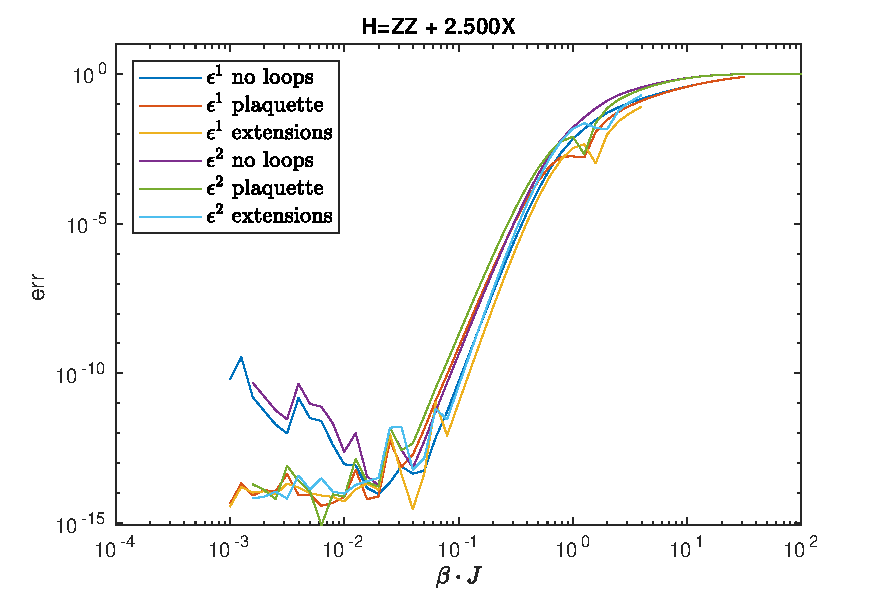
\includegraphics[width=\textwidth]{Figuren/benchmarking/2D_Err01_t_sing.pdf}
  \caption{ }
  \label{fig:res2d:n1:tising}
\end{figure}
\todo{fix caption}

\subsubsection{Heisenberg}

\subsubsection{Conclusion}

\subsection{Phase diagram 2D transveral Ising model} \label{subsec:2dpahsediag}

Now we have an idea how accurate the cluster expansions is, we can use it to calculate the thermodynamic properties of the transvere field Ising model. The sampling of points was explained in \cref{sec:phase_diag}

As a reference, \cref{2dtisingphasediag} is shown once more

\begin{figure}
  \center
  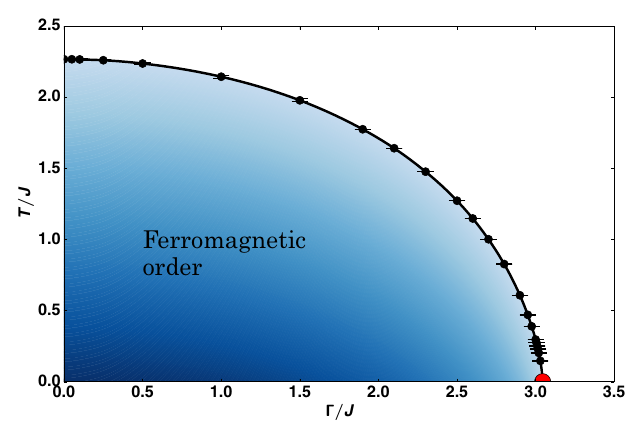
\includegraphics[width=\textwidth]{Figuren/phsyics/2disingphase.png}
  \caption{Phase diagram for 2D transversal Ising model. Figure taken from \cite{Hesselmann2016}}
  \label{2dtisingphasediag2}
\end{figure}

\subsubsection{classical Ising phase transition}
The classical ising model on a square lattice has an exact solution. Onsager calculated the critical temperature to be $T_c = \frac{2 J}{k \ln(1+\sqrt{2}) } \approx 2.69185$. A test for the construction is to simulate this and compare the fitted (see \cref{subsec:qphasediag} ) results.

At the relevant temperature, an order 5 series expansion without loops is sufficient. This keeps the bond dimension small and hence the environment can be computed faster with VUMPS.

The results are shown in \cref{fig:phase:g0:full}. Each of the figures has 4 different subplots. Left upper corner shows m vs T. For low T, there is clearly a nonzero macroscopic magnetisation, while high T has a zero expectation value as expected. The other three plots show the data collapse of the finite size scaling of the entanglement entropy $S$, the correlation length $\xi$ and the magnetisation $m$. $\delta$ is marek gap, a measure for the system size as explained in \cref{subsec:fss}.

\begin{figure}
  \center
  \includegraphics[width=\textwidth]{Figuren/phasediag/g0/Full.pdf}
  \caption{  }
  \label{fig:phase:g0:full}
\end{figure}

\todo{new figure with entropy formula fixed 6S/c instead of cS/6}

Near criticality they collapse well, but away from the critical point there is quite some systematic variation. The reason is shown in \cref{fig:crit:qtran}. Only in some limited range around the critiacal region, the universal scaling holds.

A more zoomed in version is shown in \cref{fig:phase:g0:zoomed}. Clearly. the data collapses a lot better as expected.
\begin{figure}
  \center
  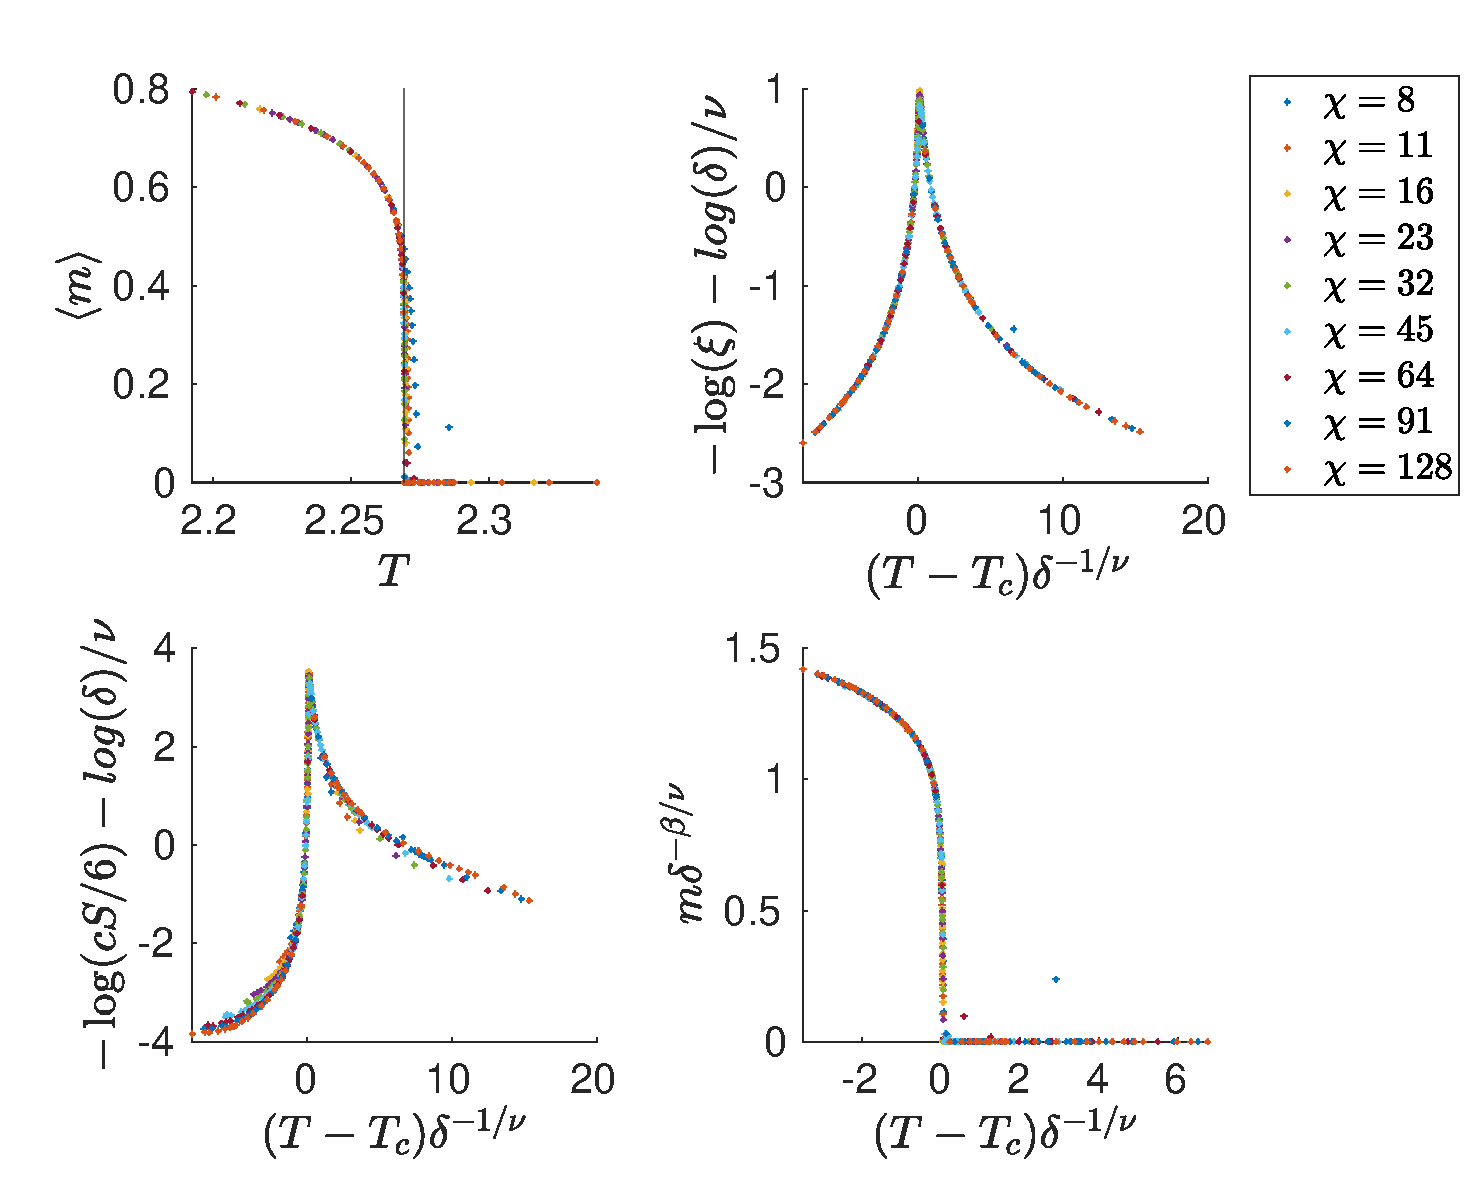
\includegraphics[width=\textwidth]{Figuren/phasediag/g0/zoomed.pdf}
  \caption{  }
  \label{fig:phase:g0:zoomed}
\end{figure}
In fact, the data collapses so well we could determine the the critical exponents and the temperature with the given data.

\todo{provide numbers for fit}

\subsubsection{g=2.5 phase transition }

The previous example simulated the classical 2D ising model. The question is whether this result will carry on into the quantum regime.The results for the full phase diagram \cref{fig:phase:g25:full} and or points in direct neighbourhood of the phase transition \cref{fig:phase:g25:zoomed} are similar to the 1D case.

Of course, quantitive details are different: the phase transition happens at $T\approx 1.274$ and the maximum magnetisation is lower than 1, in accordance to \cref{2dtisingphasediag}. The variation of m around the critical temperature for different bond dimensions is much higher. A much larger $\chi$ is needed for the fixed point MPS. This is not necessarily a problem, as this gives better data for the finite size scaling.

\begin{figure}
  \center
  \includegraphics[width=\textwidth]{Figuren/phasediag/g25/Full.pdf}
  \caption{  }
  \label{fig:phase:g25:full}
\end{figure}

\begin{figure}
  \center
  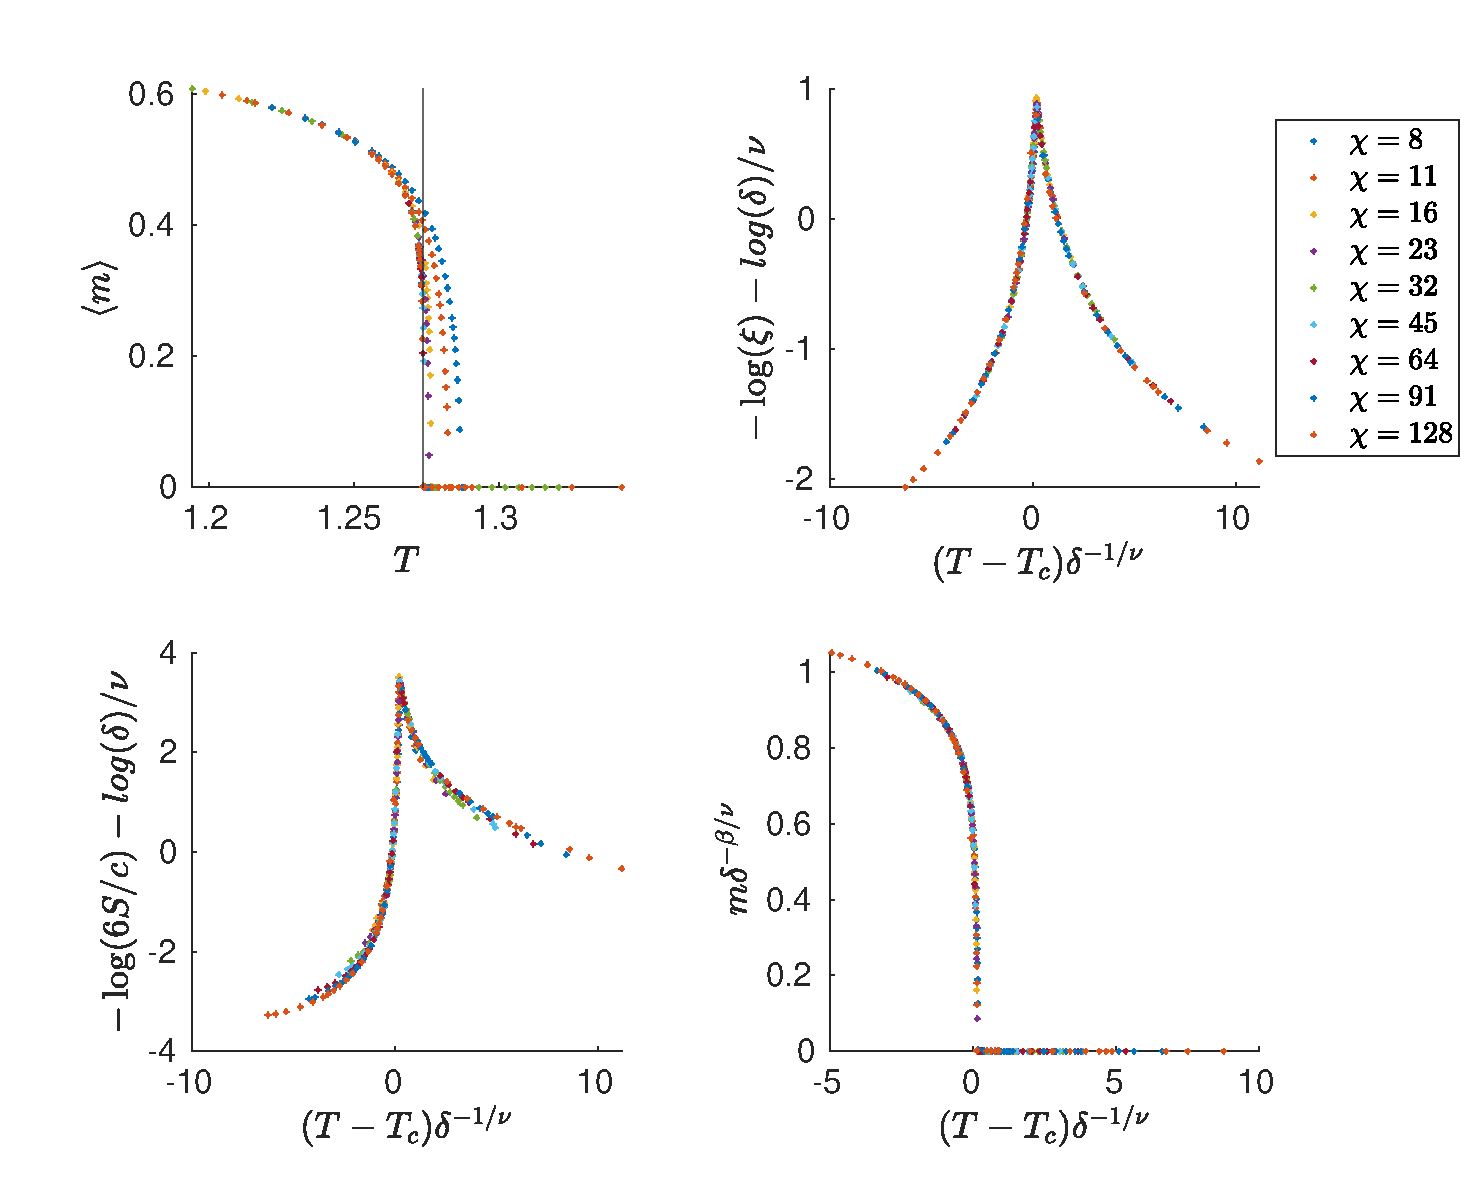
\includegraphics[width=\textwidth]{Figuren/phasediag/g25/zoomed.pdf}
  \caption{  }
  \label{fig:phase:g25:zoomed}
\end{figure}

There is no analytical expression for critical temperature known. With quantum monte carlo techniques, a value of $T_c=1.2737(6)$ is obtained, while state of the art tensor network techniques provide a value of $T_c=1.2737(2)$ \cite{Czarnik2019}

With the series expansion from this paper and Vumps, $T_c=1.2736(6)$, indicating that this faithfully captures the physics. To put his into context: the directly calculated error $\epsilon^{2}$  at $T=1.2$ was around $0.006$.

\subsubsection{ T=0.7 quantum phase transition }\label{tphasetranssubsec}

Up untill now, the phase diagram in \cref{2dtisingphasediag2} was explored at constant g in function of T, but of course there is also a transition at constant T and varying g.  T = 0.7 is chosen. The results are shown in \cref{fig:phase:t07:full}.

\begin{figure}
  \center
  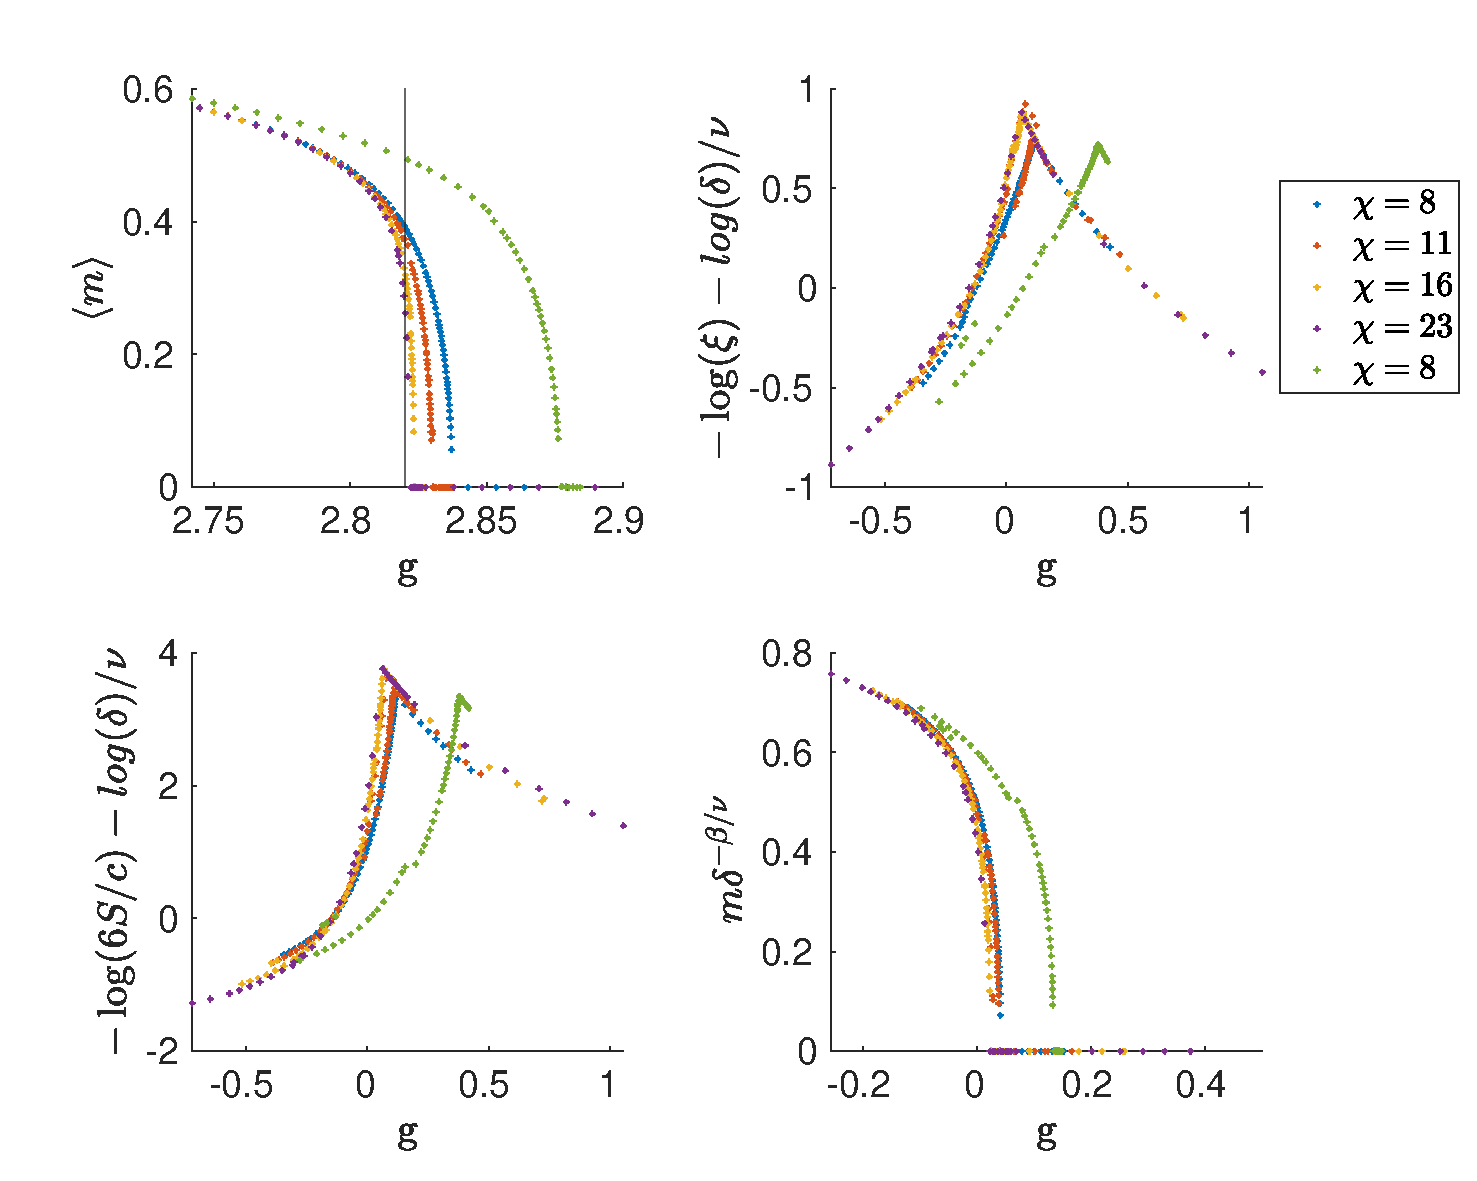
\includegraphics[width=\textwidth]{Figuren/phasediag/t07/full.pdf}
  \caption{Results for $T=0.7$ phase transition. The green points are a truncated order 6 construction, the others order 5.  }
  \label{fig:phase:t07:full}
\end{figure}

Clearly, the results do not collapse as well as for the other models. The reason is that the order of the expension is not high enough. The green curve is order 6, where virtual level is truncated to dimension 20. The others are order 5. The green and blue curve both have MPS bond dimension $\chi=8$, but predict quit different magnetisation fpr large g. This shows that for $g>0.7$, order 5 is not sufficient anymore.

\subsubsection{Tricritical point}

Now that we know the critical transveral field can be determined, all the tools are present to extrapolate the Tricritical point, indicated by a red dot in \cref{2dtisingphasediag2}. To achieve this, the following scaling relation can be used:
\begin{equation}
  T_c = \left| g_c-g_{c,q} \right|^{z \nu_{3D}}
\end{equation}
Near the critical point, the critical temperature $T_c$ and the critical transversal field $g_c$ are related to each other by the value of the quantum critical point $g_{c,q}$ and critical exponent $z=1$ and $\nu_{3D} \approx 0.62998$ \cite{Hesselmann2016}.

This could perfectly be done, given enough computation time to calculate for many temperatures the critical transversal field with a finite size scaling, similar to \cref{tphasetranssubsec}. Possibly, also a scaling in truncation dimension for the cluster expansion is needed.

\subsection{Going beyond }
With all the built machinery to construct cluster expansions, is logical to calculate the phase diagram with increased precision.

\subsubsection{loops and extensions}
Adding loops decreases the error. but there is also a surprising result: all possible loop extensions result in a higher error. The fluctuation increases drastically. With increasing bond dimension $\chi$, this is somewhat better but still not good enough.
The question is wether this is a result of a failing cluster expansion, or inability VUMPS to calculate the correct environment. During my thesis, my focus has largely been on the first case. After all, the framework was completely build from scratch and errors happen, and there is no guarantee that the series even converges. But introduction of very strict variants, such as the generalization to type E, where left/upper extension have level a and the right/lower extensions are of type a':
\begin{equation}
  \vcenter{ \hbox{  \pepob{5}{3}{{
            "-","-","-","-",
            "-","a","$\alpha$","-",
            "-","-","$\alpha$","-"}}{{
            "-","-",
            "-","-",
            "-","$\alpha$",
            "-","$\alpha$",
            "-","-"}}{{
            1,1,1,1,1,
            1,0,0,0,1,
            1,1,0,0,1}} }} \\
  \vcenter{ \hbox{  \pepob{5}{3}{{
            "-","-","-","-",
            "-","0","$\alpha$","-",
            "-","-","$\alpha$","-"}}{{
            "-","-",
            "-","-",
            "a'","$\alpha$",
            "-","$\alpha$",
            "-","-"}}{{
            1,1,0,1,1,
            1,1,0,0,1,
            1,1,0,0,1}} }}
\end{equation}
Introduce these variations.

The VUMPS producedure come with 2 implicit assumptions: the original version was derived for hermitian hamiltonians. The MPO resulting from the traced PEPO  from the culster expansion is not an hermition MPO.

A second assumption made during this thesis is that the wave function can be represented by a 1by1 unit cell. Despite efforts made, the multisite version \cite{Nietner2020} doesn't seem to produce sensible results, even for version where 1by1 unit cell does give the right results.

It's clear that more research is needed here. One way to locate the problem would be to use another algorithm to contract the network, such as corner transfer matrix renormalization group (CTMRG) as used in  cite{Czarnik2019}, or even using the single site VUMPS algorithm combined with blocking:

\begin{equation}
  \vcenter{ \hbox{  \pepob{4}{4}{{
            "","-","",
            "","","",
            "","","",
            "","-","",}}{{
            "","-","",
            "","","",
            "","","",
            "","-","",}}{{
            1,4,4,1,
            4,0,0,4,
            4,0,0,4,
            1,4,4,1}} }} \cong  \vcenter{ \hbox{  \pepob{3}{3}{{
            "","",
            "","",
            "","",}}{{
            "","","",
            "","","",}}{{
            1,4,1,
            4,0,4,
            1,4,1}} }}
\end{equation}

\todo{complex matrices instead of real ones??}

\subsubsection{Higher order}

Going to higher order (i.e. longer linear chains) and adding the single loop contribution works well. The bond dimension of largest virtual level (3 in this case) can be truncated in the construction. The linear and non-linear solver find the least squares solution to the problems.

Care has to be taken in order to not violate one of the conclusions in 1D: never construct a longer chain than the previously fully solved one. For instance if the bond is truncated to 10, the linear chains can be constructed up till order 4. This means \cref{eq:cross_terms:order4} can be added but not \cref{eq:cross_terms:order5}, because the longest chains are order 5. Level 5 can still be constructed and contracted easily, but virtual level 3 has a bond dimension of 64. Compared to the previous bond dimensions (1,4 and 16) this is quite large and needs to be truncated.

\subsubsection{Better extrapolation}

The spirit behind finite size scaling is to calculate more with the data availalbe. In \cref{subsec:fss}, 2 additional varariations were suggested. One is to account for the subleading finite size corrections, the other to cange the way of calculating $\delta$.

\paragraph{subleading corrections}
Intruducing subleading corrections requires 4 parameters for each fitted universal function: $\omega$,$\phi$,$c$ and $d$ from \cref{ea:subleadparam}. Compared to the one parameter $T_c$ or $g_c$, this is a lot and can be used to make many graphs collapse into a singlge graph. The analysis in \cite{Wang2006} curefully estimates the error made with the fitting procedure. A similar amount of rigour would be required to fully trust the results.

Nevertheless, fitting with subleading corrections results in critical temperatures close to the ones fitted without, and the subleading exponents are close to 1, as expected from the subleading series expansion.

\paragraph{ Choice  $\delta$  }

Different choices of $c_i$ in \cref{eq:cit_delta} are possible to construct $\delta$.  Variantional optimisation was doen as suggested in \cite{Nietner2020}. Both the x and y axis should be normalised, because depending on $\delta$ the scale changes. If scaled based on the outer points, there is a flaw in the fitting procedure.  The variational minimum goes to a point where at least for one point $\delta$ is extremely close to 0, and hence everything on the x axis except that point is pinched together, resulting in very small relative error. Therefore, it is better to normalise according to the points a e.g. 25th percentile and 75th percentile of the range on the  axis.

This improves the collapse, but is not clear how much the prediction of $T_c$ or $g_c$ is improved.

\section{Conclusion}

The results in previous section show that this novel method can compete against some recent tensor network results in literature.